\chapter{Budowanie funkcji logicznych (NAND)}

    \section{NOT}
        \begin{itemize}
            \item Zbudowany układ wraz ze schematem oraz rozpiską pinów:
                \begin{figure}[H]
                    \centering
                    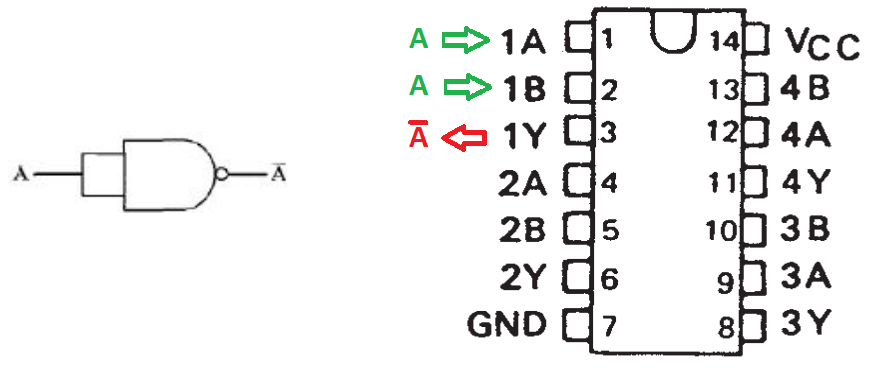
\includegraphics[width=0.5\textwidth]{img/schemes_with_pins/NAND_not_w_pins.png}
                    \label{NAND:schemat_not_w_pins}
                \end{figure}
                \begin{figure}[H]
                    \centering
                    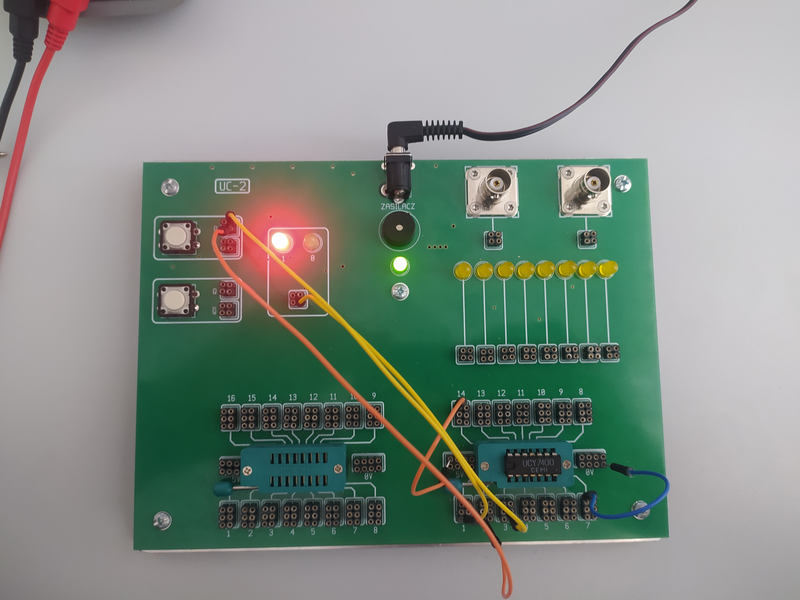
\includegraphics[width=0.5\textwidth]{img/NAND/funkcje/1652306732632_scaled.png}
                    \caption{Zbudowany układ}
                    \label{NAND:zbudowany_układ_NOT}
                \end{figure}
            \item Sprawdzanie stanów:
                \begin{figure}[H]
                    \centering
                        \begin{subfigure}[h]{0.35\textwidth}
                            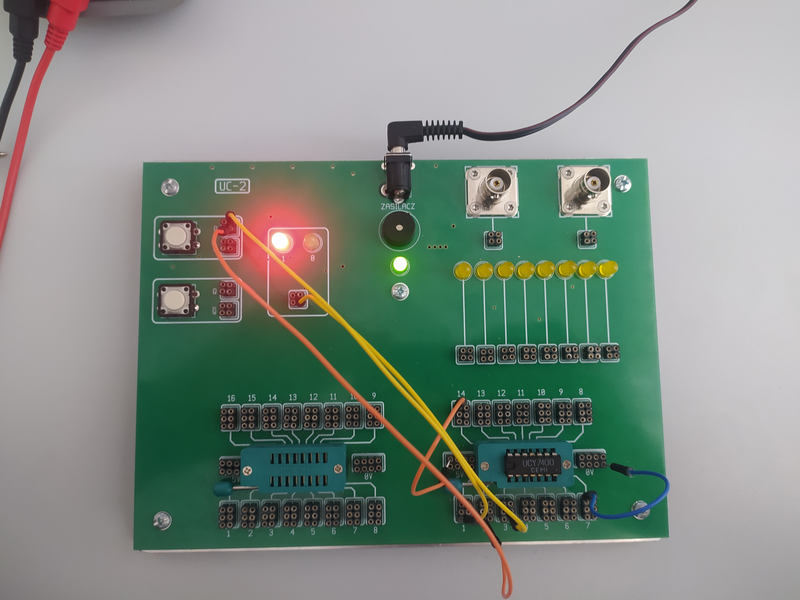
\includegraphics[width=\textwidth]{img/NAND/funkcje/1652306732632_scaled.png}
                        \end{subfigure}
                        \begin{subfigure}[h]{0.35\textwidth}
                            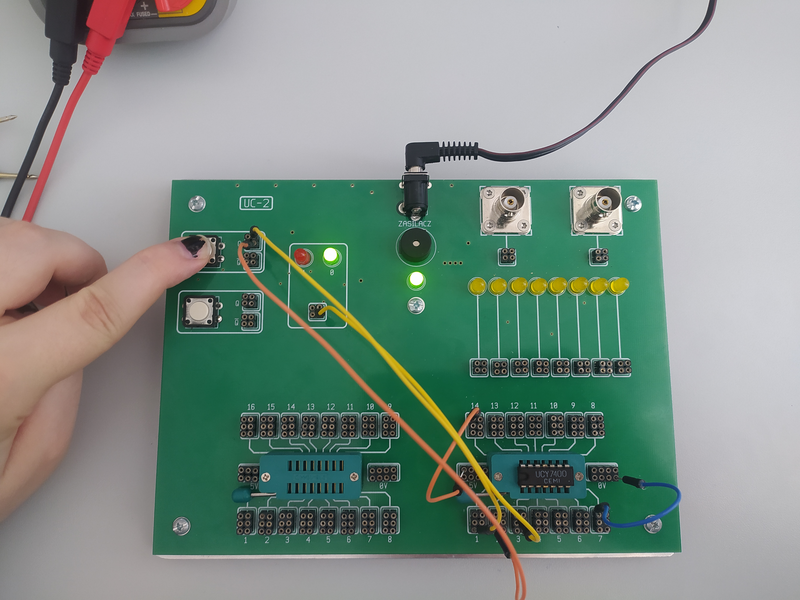
\includegraphics[width=\textwidth]{img/NAND/funkcje/1652306732620_scaled.png}
                        \end{subfigure}
                    \label{NAND:testy_NOT}
                \end{figure}
            \item Tabela stanów:
                \begin{center}
                    \label{NAND:tabela_prawdy_NOT}
                    \begin{tabular}{|c|>{\columncolor[gray]{0.8}}c|}
                        \hline
                        A & Y \\
                        \hline
                        0 & 1 \\
                        \hline
                        1 & 0 \\
                        \hline
                    \end{tabular}
                \end{center}
            \item Zbudowany układ \textbf{poprawnie} reaguje na przesyłane sygnały (zgodnie z teoretycznymi przewidywaniami \ref{tabela_prawdy:NOT})
        \end{itemize}
    
\pagebreak

    \section{OR}
        \begin{itemize}
            \item Zbudowany układ wraz ze schematem oraz rozpiską pinów:
                \begin{figure}[H]
                    \centering
                    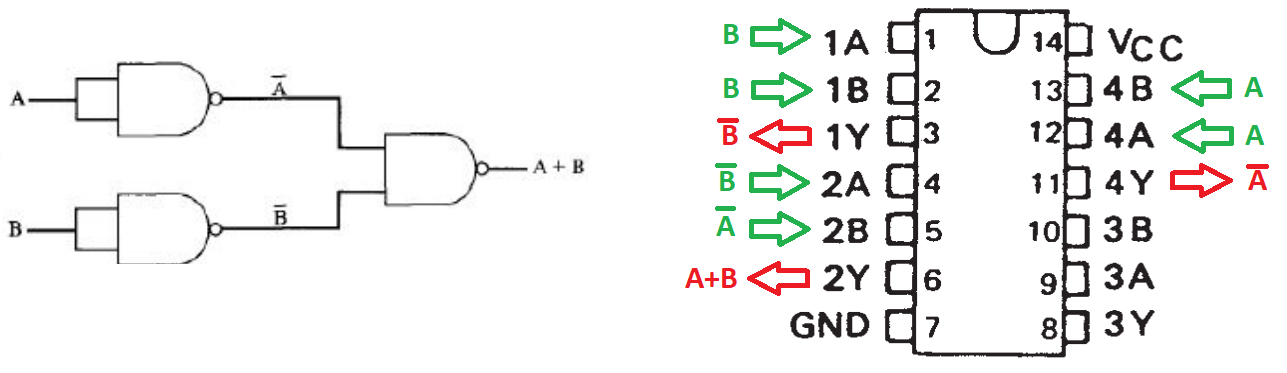
\includegraphics[width=\textwidth]{img/schemes_with_pins/NAND_or_w_pins.png}
                    \label{NAND:schemat_or_w_pins}
                \end{figure}
                \begin{figure}[H]
                    \centering
                    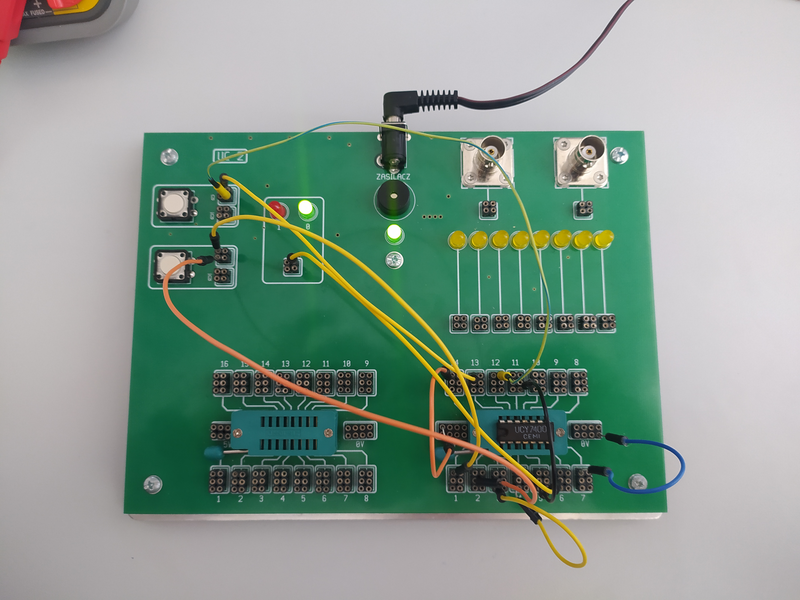
\includegraphics[width=\textwidth]{img/NAND/funkcje/1652306732527_scaled.png}
                    \caption{Zbudowany układ}
                    \label{NAND:zbudowany_układ_OR}
                \end{figure}
                        
            \pagebreak
            
            \item Sprawdzanie stanów:
                \begin{figure}[H]
                    \centering
                        \begin{subfigure}[h]{0.4\textwidth}
                            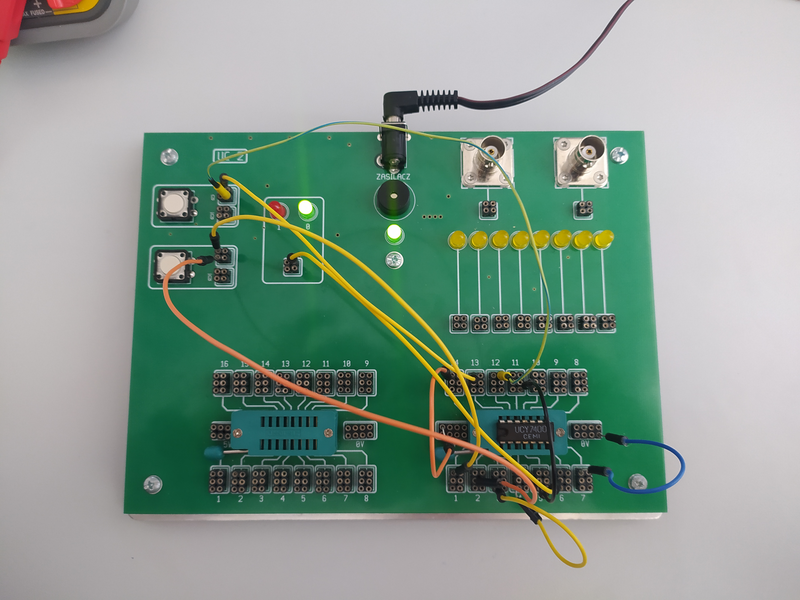
\includegraphics[width=\textwidth]{img/NAND/funkcje/1652306732527_scaled.png}
                        \end{subfigure}
                        \begin{subfigure}[h]{0.4\textwidth}
                            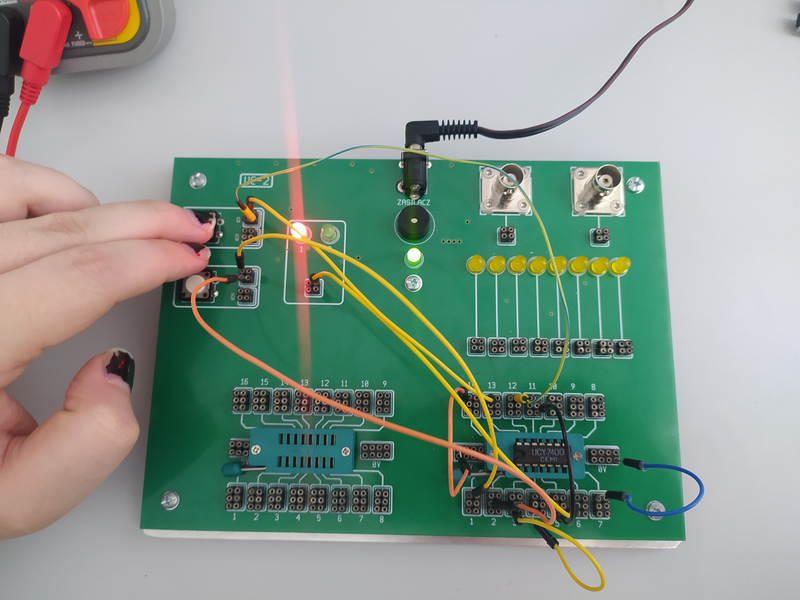
\includegraphics[width=\textwidth]{img/NAND/funkcje/1652306732517_scaled.png}
                        \end{subfigure}
                        \begin{subfigure}[h]{0.4\textwidth}
                            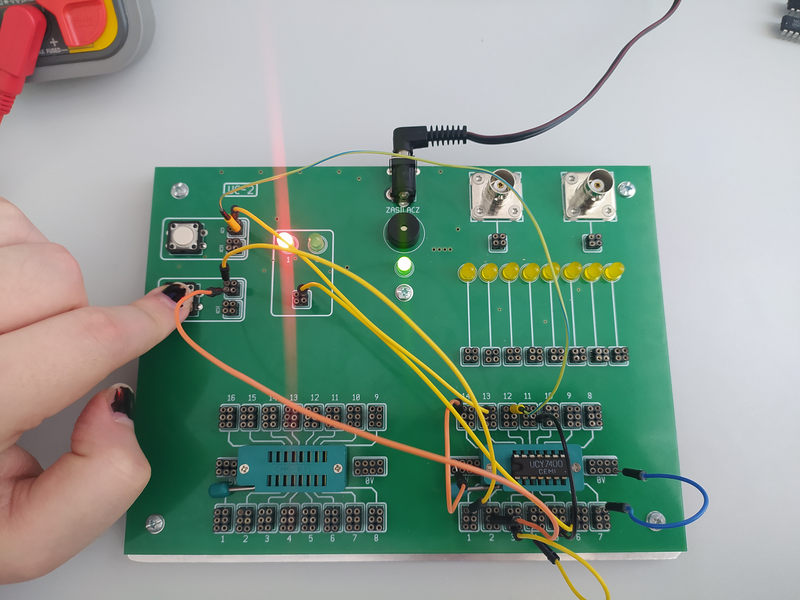
\includegraphics[width=\textwidth]{img/NAND/funkcje/1652306732506_scaled.png}
                        \end{subfigure}
                        \begin{subfigure}[h]{0.4\textwidth}
                            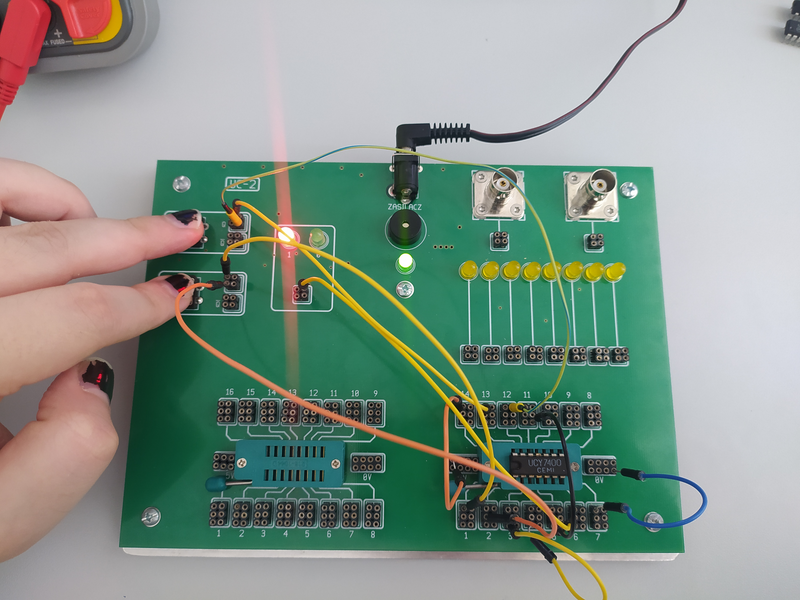
\includegraphics[width=\textwidth]{img/NAND/funkcje/1652306732496_scaled.png}
                        \end{subfigure}
                    \label{NAND:testy_OR}
                \end{figure}
            \item Tabela stanów:
                \begin{center}
                    \label{NAND:tabela_prawdy_OR}
                    \begin{tabular}{|c|c|>{\columncolor[gray]{0.8}}c|}
                        \hline
                        A & B & Y \\
                        \hline
                        0 & 0 & 0 \\
                        \hline
                        0 & 1 & 1 \\
                        \hline
                        1 & 0 & 1 \\
                        \hline
                        1 & 1 & 1 \\
                        \hline
                    \end{tabular}
                \end{center}
            \item Zbudowany układ \textbf{poprawnie} reaguje na przesyłane sygnały (zgodnie z teoretycznymi przewidywaniami \ref{tabela_prawdy:OR})
        \end{itemize}
        
\pagebreak

    \section{AND}
        \begin{itemize}
            \item Zbudowany układ wraz ze schematem oraz rozpiską pinów:
                \begin{figure}[H]
                    \centering
                    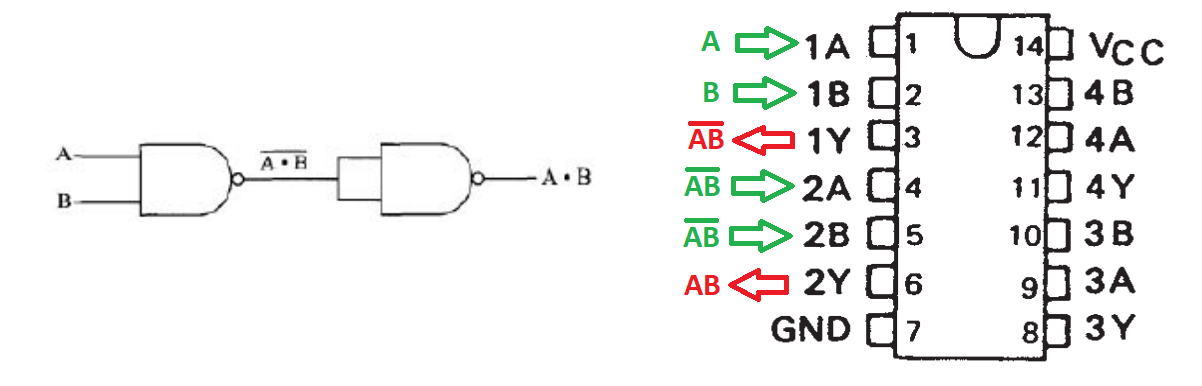
\includegraphics[width=\textwidth]{img/schemes_with_pins/NAND_and_w_pins.png}
                    \label{NAND:schemat_and_w_pins}
                \end{figure}
                \begin{figure}[H]
                    \centering
                    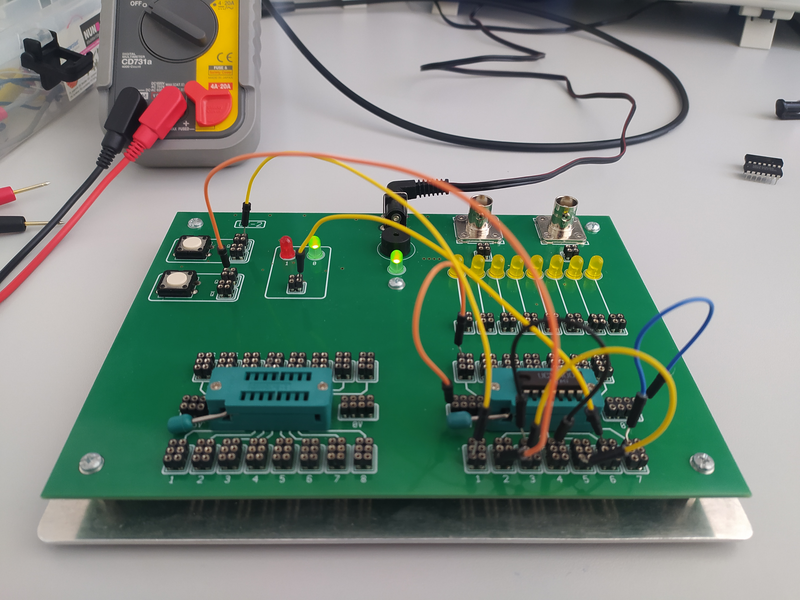
\includegraphics[width=\textwidth]{img/NAND/funkcje/1652306732610_scaled.png}
                    \caption{Zbudowany układ}
                    \label{NAND:zbudowany_układ_AND}
                \end{figure}
                
            \pagebreak
                
            \item Sprawdzanie stanów:
                \begin{figure}[H]
                    \centering
                        \begin{subfigure}[h]{0.4\textwidth}
                            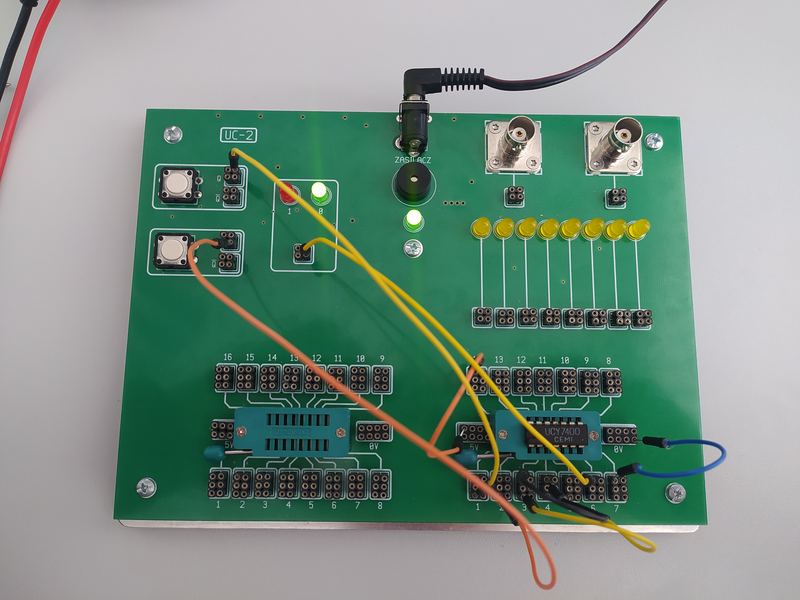
\includegraphics[width=\textwidth]{img/NAND/funkcje/1652306732595_scaled.png}
                        \end{subfigure}
                        \begin{subfigure}[h]{0.4\textwidth}
                            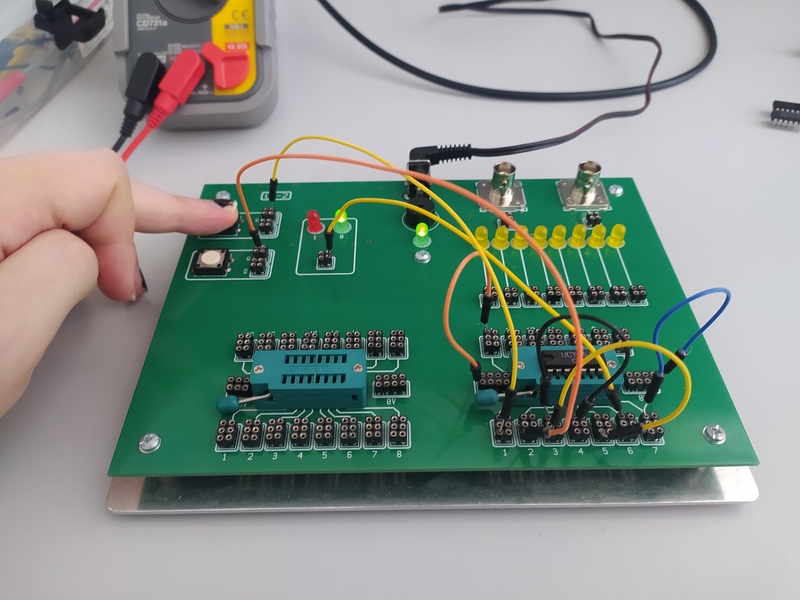
\includegraphics[width=\textwidth]{img/NAND/funkcje/1652306732585_scaled.png}
                        \end{subfigure}
                        \begin{subfigure}[h]{0.4\textwidth}
                            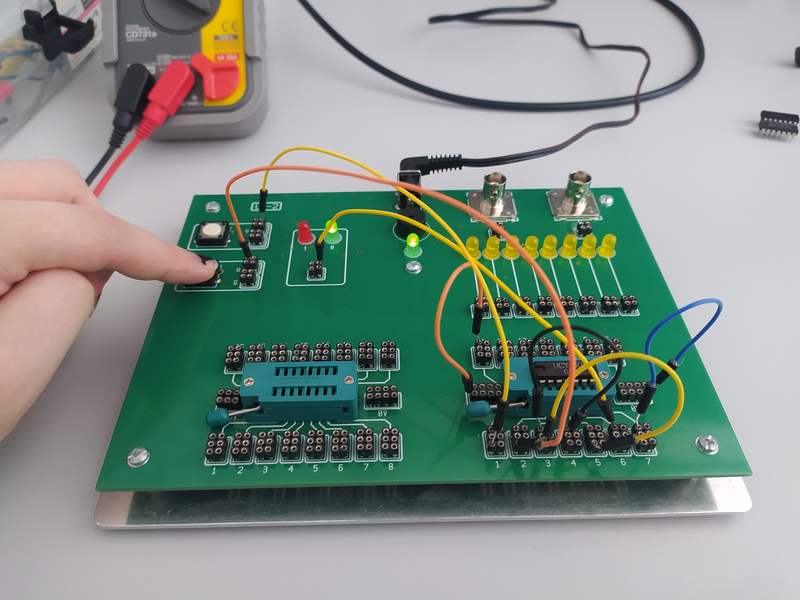
\includegraphics[width=\textwidth]{img/NAND/funkcje/1652306732564_scaled.png}
                        \end{subfigure}
                        \begin{subfigure}[h]{0.4\textwidth}
                            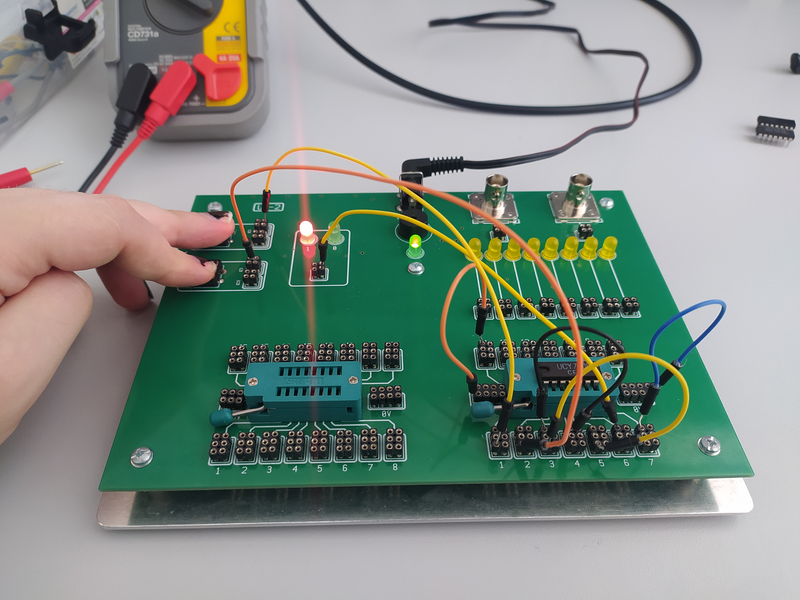
\includegraphics[width=\textwidth]{img/NAND/funkcje/1652306732552_scaled.png}
                        \end{subfigure}
                    \label{NAND:testy_AND}
                \end{figure}
            \item Tabela stanów:
                \begin{center}
                    \label{NAND:tabela_prawdy_AND}
                    \begin{tabular}{|c|c|>{\columncolor[gray]{0.8}}c|}
                        \hline
                        A & B & Y \\
                        \hline
                        0 & 0 & 0 \\
                        \hline
                        0 & 1 & 0 \\
                        \hline
                        1 & 0 & 0 \\
                        \hline
                        1 & 1 & 1 \\
                        \hline
                    \end{tabular}
                \end{center}
            \item Zbudowany układ \textbf{poprawnie} reaguje na przesyłane sygnały (zgodnie z teoretycznymi przewidywaniami \ref{tabela_prawdy:AND})
    \end{itemize}

\pagebreak

\chapter{Budowanie funkcji logicznych (NOR)}

    \section{NOT}
        \begin{itemize}
            \item Zbudowany układ wraz ze schematem oraz rozpiską pinów:
                \begin{figure}[H]
                    \centering
                    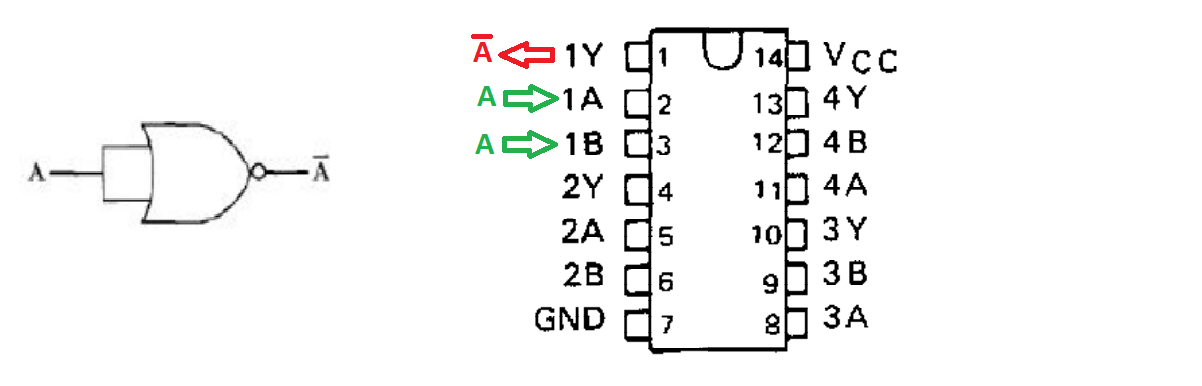
\includegraphics[width=0.5\textwidth]{img/schemes_with_pins/NOR_not_w_pins.png}
                    \label{NOR:schemat_not_w_pins}
                \end{figure}
                \begin{figure}[H]
                    \centering
                    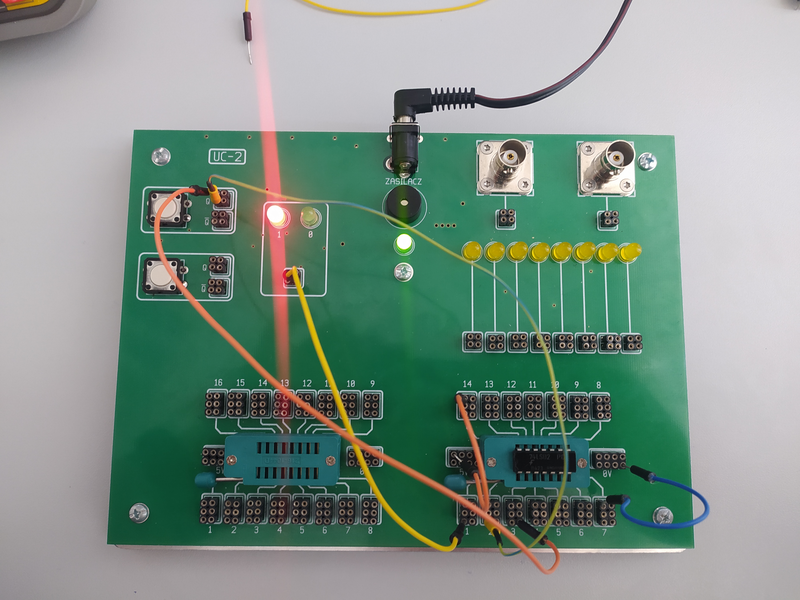
\includegraphics[width=0.5\textwidth]{img/NOR/funkcje/1652306732483_scaled.png}
                    \caption{Zbudowany układ}
                    \label{NOR:zbudowany_układ_NOT}
                \end{figure}
            \item Sprawdzanie stanów:
                \begin{figure}[H]
                    \centering
                        \begin{subfigure}[h]{0.4\textwidth}
                            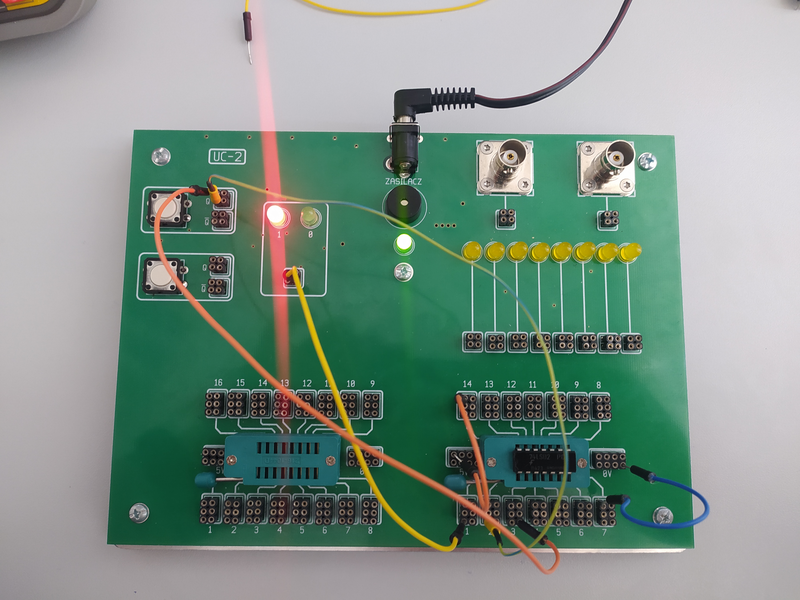
\includegraphics[width=\textwidth]{img/NOR/funkcje/1652306732483_scaled.png}
                        \end{subfigure}
                        \begin{subfigure}[h]{0.4\textwidth}
                            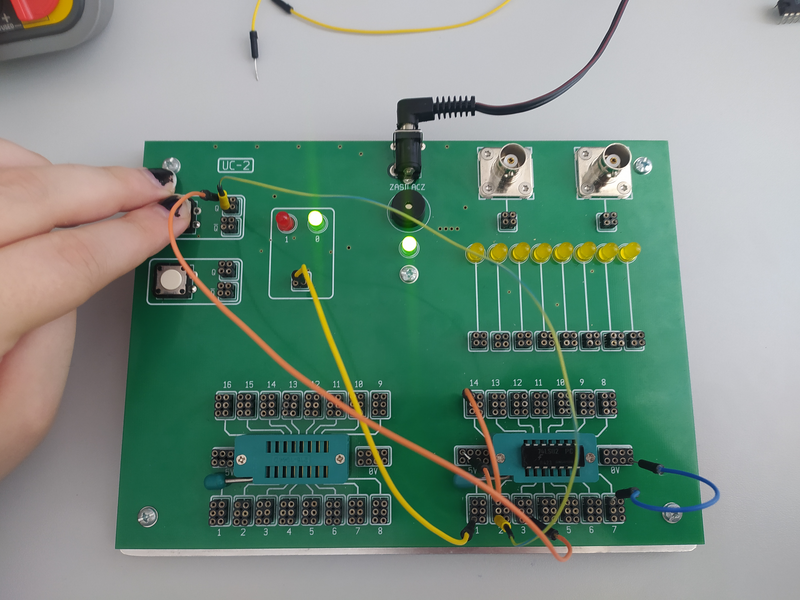
\includegraphics[width=\textwidth]{img/NOR/funkcje/1652306732471_scaled.png}
                        \end{subfigure}
                    \label{NOR:testy_NOT}
                \end{figure}
            \item Tabela stanów:
                \begin{center}
                    \label{NOR:tabela_prawdy_NOT}
                    \begin{tabular}{|c|>{\columncolor[gray]{0.8}}c|}
                        \hline
                        A & Y \\
                        \hline
                        0 & 1 \\
                        \hline
                        1 & 0 \\
                        \hline
                    \end{tabular}
                \end{center}
            \item Zbudowany układ \textbf{poprawnie} reaguje na przesyłane sygnały (zgodnie z teoretycznymi przewidywaniami \ref{tabela_prawdy:NOT})
        \end{itemize}


\pagebreak
    
    \section{OR}
        \begin{itemize}
            \item Zbudowany układ wraz ze schematem oraz rozpiską pinów:
                \begin{figure}[H]
                    \centering
                    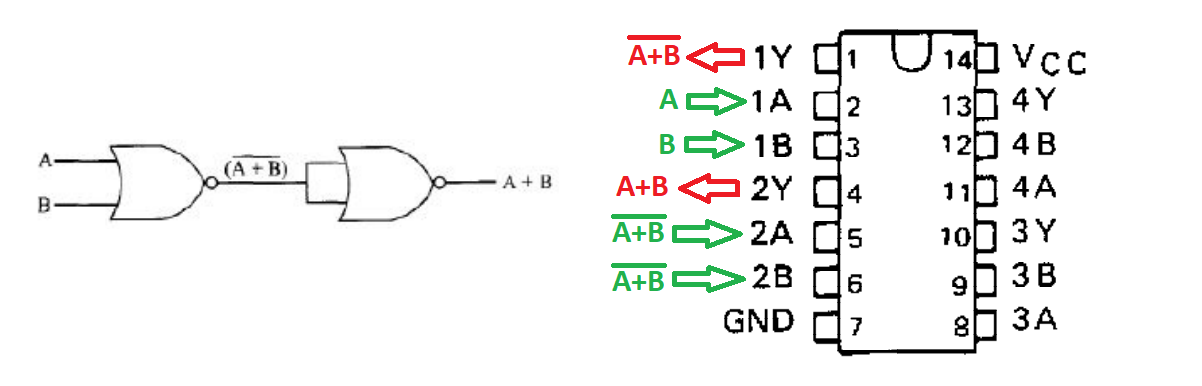
\includegraphics[width=\textwidth]{img/schemes_with_pins/NOR_or_w_pins.png}
                    \label{NOR:schemat_or_w_pins}
                \end{figure}
                \begin{figure}[H]
                    \centering
                    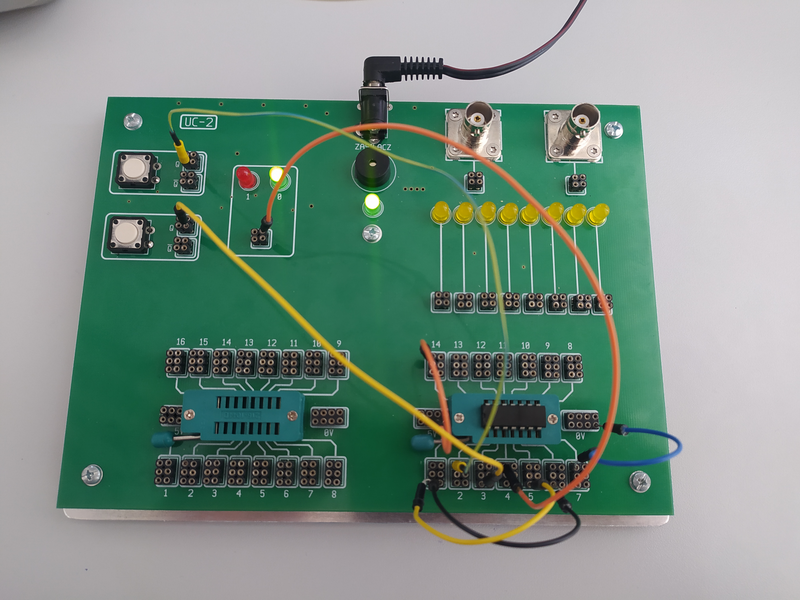
\includegraphics[width=\textwidth]{img/NOR/funkcje/1652306732459_scaled.png}
                    \caption{Zbudowany układ}
                    \label{NOR:zbudowany_układ_OR}
                \end{figure}
                
        \pagebreak            
                    
            \item Sprawdzanie stanów:
                \begin{figure}[H]
                    \centering
                        \begin{subfigure}[h]{0.4\textwidth}
                            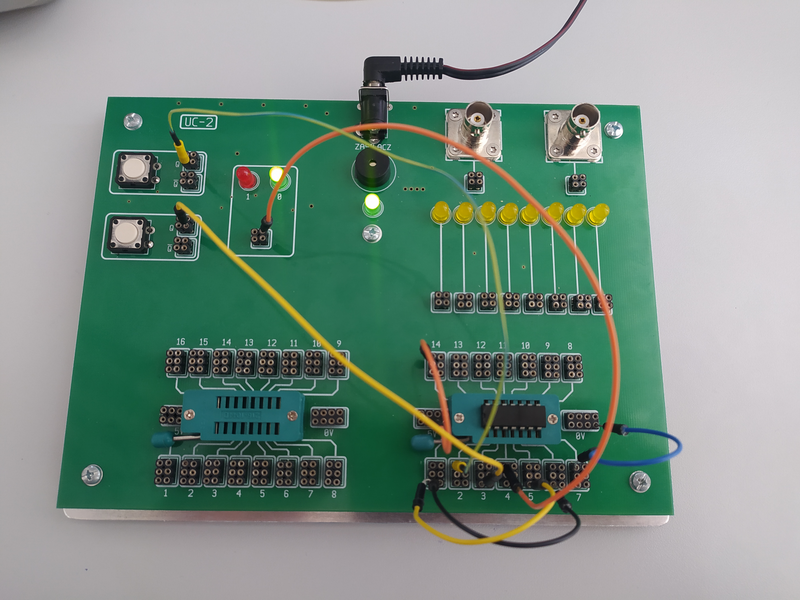
\includegraphics[width=\textwidth]{img/NOR/funkcje/1652306732459_scaled.png}
                        \end{subfigure}
                        \begin{subfigure}[h]{0.4\textwidth}
                            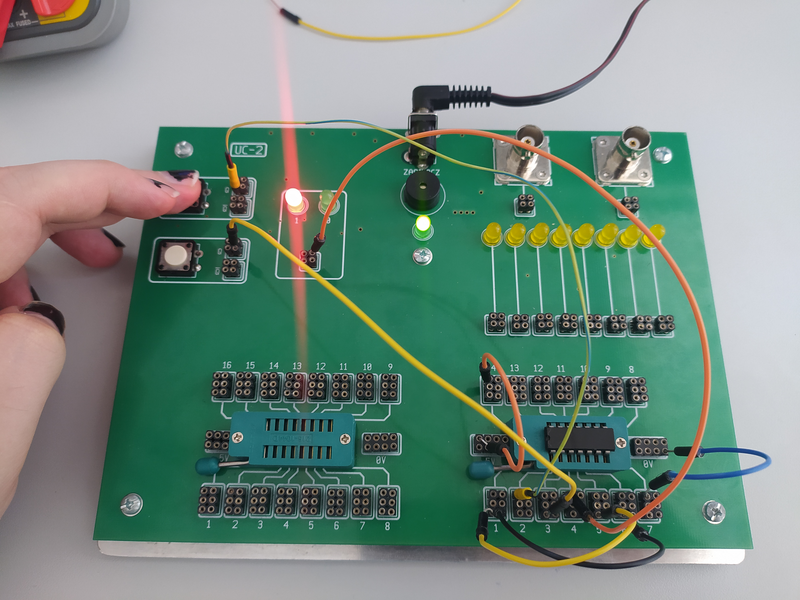
\includegraphics[width=\textwidth]{img/NOR/funkcje/1652306732450_scaled.png}
                        \end{subfigure}
                        \begin{subfigure}[h]{0.4\textwidth}
                            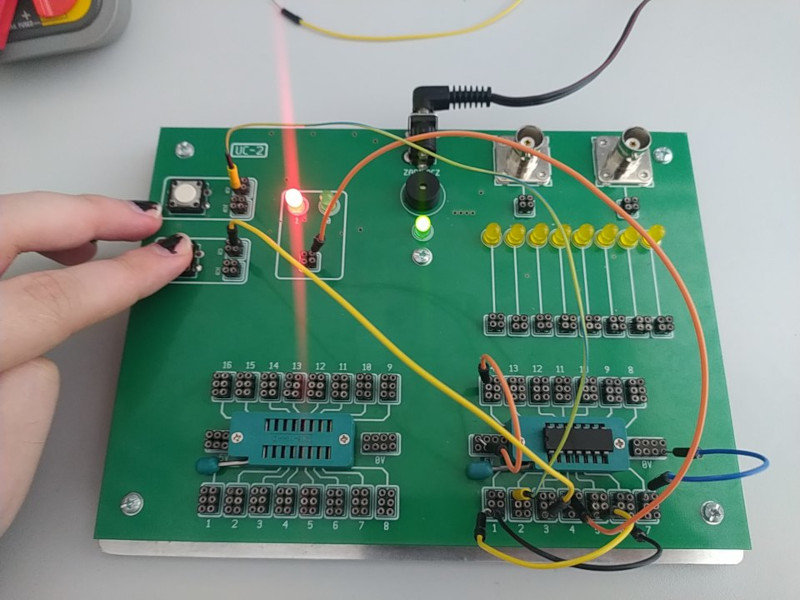
\includegraphics[width=\textwidth]{img/NOR/funkcje/1652306732442_scaled.jpg}
                        \end{subfigure}
                        \begin{subfigure}[h]{0.4\textwidth}
                            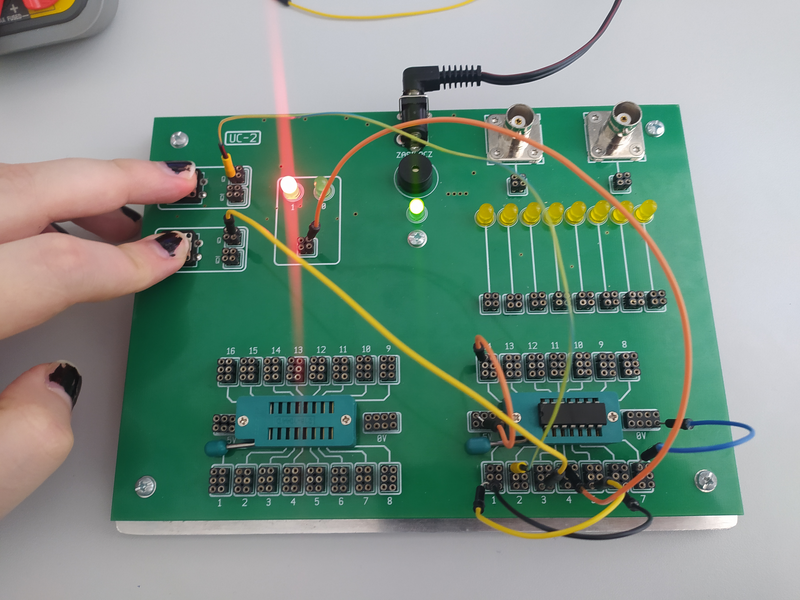
\includegraphics[width=\textwidth]{img/NOR/funkcje/1652306732434_scaled.png}
                        \end{subfigure}
                    \label{NOR:testy_OR}
                \end{figure}
            \item Tabela stanów:
                \begin{center}
                    \label{NOR:tabela_prawdy_OR}
                    \begin{tabular}{|c|c|>{\columncolor[gray]{0.8}}c|}
                        \hline
                        A & B & Y \\
                        \hline
                        0 & 0 & 0 \\
                        \hline
                        0 & 1 & 1 \\
                        \hline
                        1 & 0 & 1 \\
                        \hline
                        1 & 1 & 1 \\
                        \hline
                    \end{tabular}
                \end{center}
            \item Zbudowany układ \textbf{poprawnie} reaguje na przesyłane sygnały (zgodnie z teoretycznymi przewidywaniami \ref{tabela_prawdy:OR})
        \end{itemize}
        
\pagebreak
        
    \section{AND}
            
        \begin{itemize}
            \item Zbudowany układ wraz ze schematem oraz rozpiską pinów:
                \begin{figure}[H]
                    \centering
                    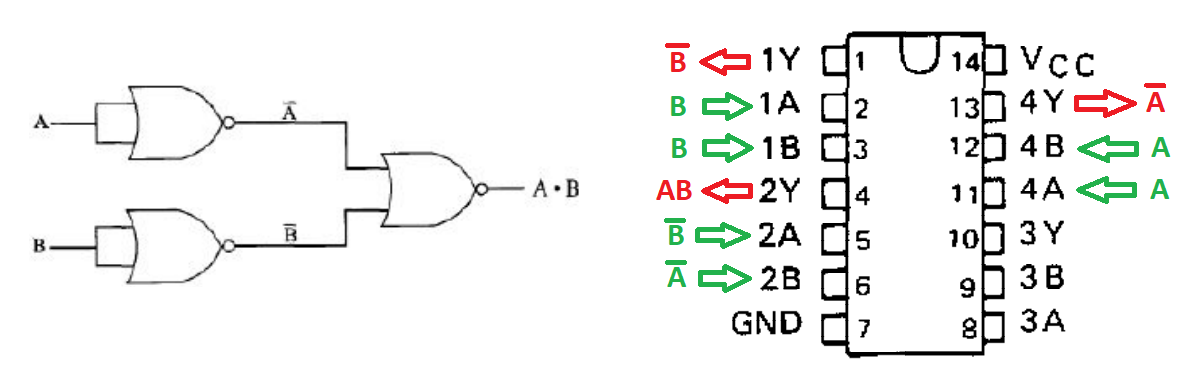
\includegraphics[width=\textwidth]{img/schemes_with_pins/NOR_and_w_pins.png}
                    \label{NOR:schemat_and_w_pins}
                \end{figure}
                \begin{figure}[H]
                    \centering
                    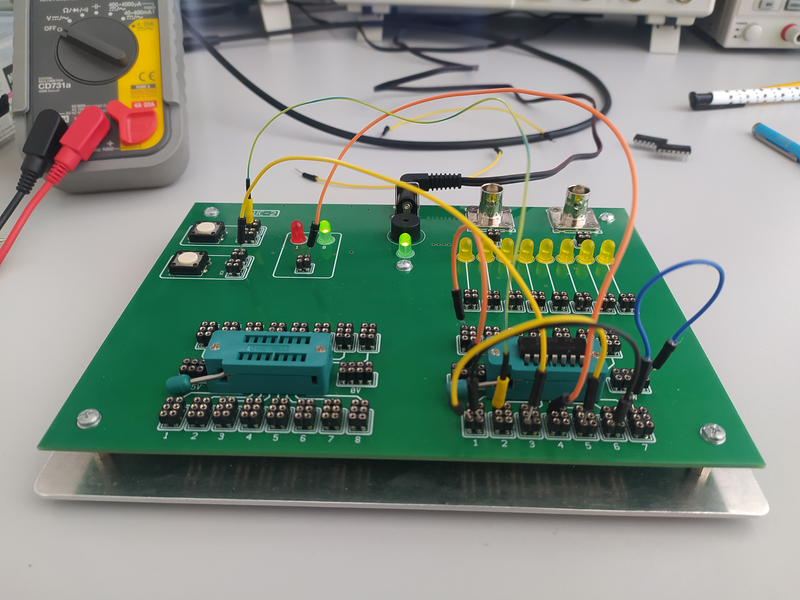
\includegraphics[width=\textwidth]{img/NOR/funkcje/1652306732425_scaled.png}
                    \caption{Zbudowany układ}
                    \label{NOR:zbudowany_układ_AND}
                \end{figure}
                    
            \pagebreak        
                    
            \item Sprawdzanie stanów:
                \begin{figure}[H]
                    \centering
                        \begin{subfigure}[h]{0.4\textwidth}
                            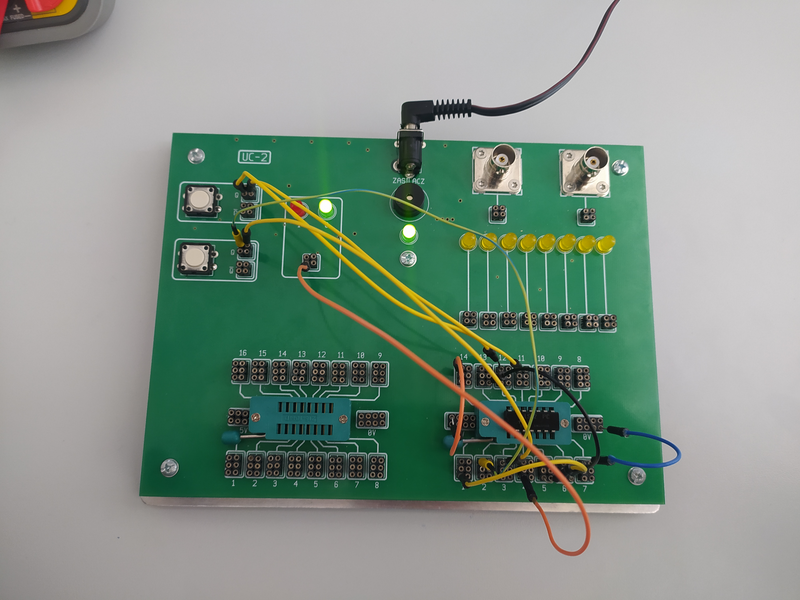
\includegraphics[width=\textwidth]{img/NOR/funkcje/1652306732408_scaled.png}
                        \end{subfigure}
                        \begin{subfigure}[h]{0.4\textwidth}
                            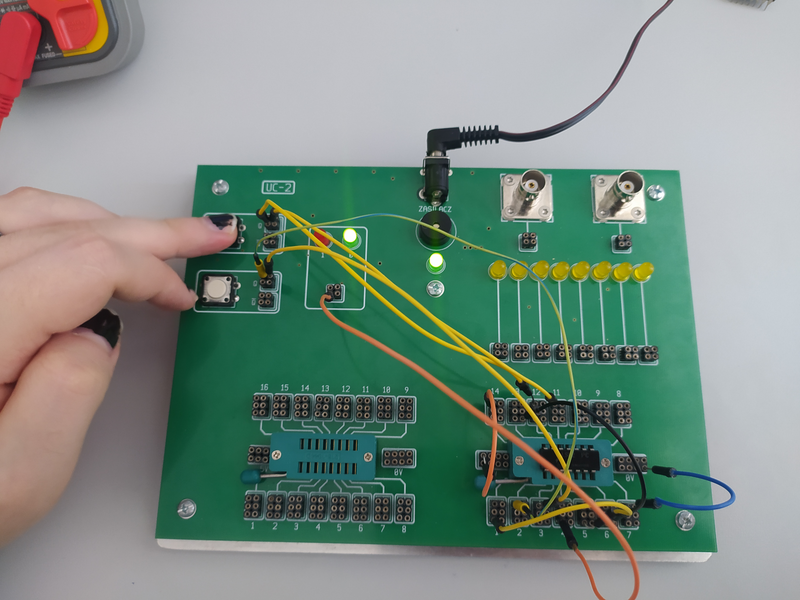
\includegraphics[width=\textwidth]{img/NOR/funkcje/1652306732399_scaled.png}
                        \end{subfigure}
                        \begin{subfigure}[h]{0.4\textwidth}
                            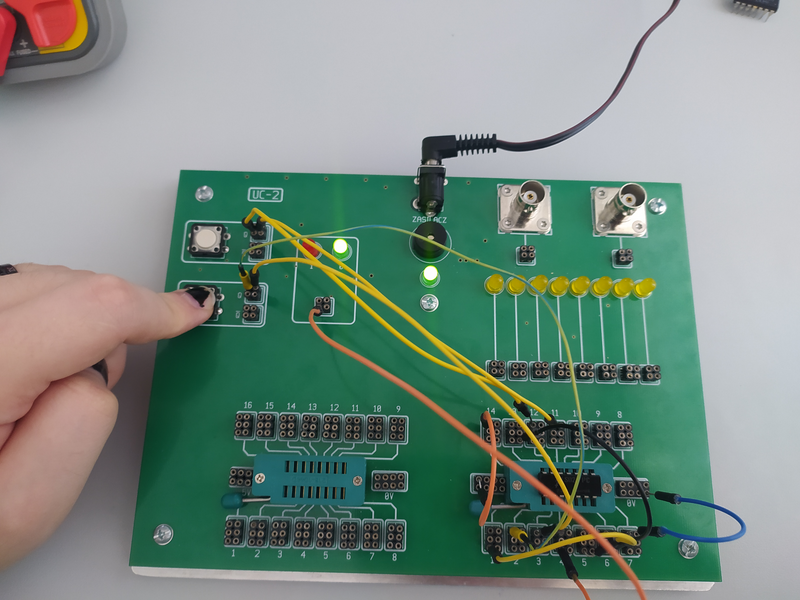
\includegraphics[width=\textwidth]{img/NOR/funkcje/1652306732390_scaled.png}
                        \end{subfigure}
                        \begin{subfigure}[h]{0.4\textwidth}
                            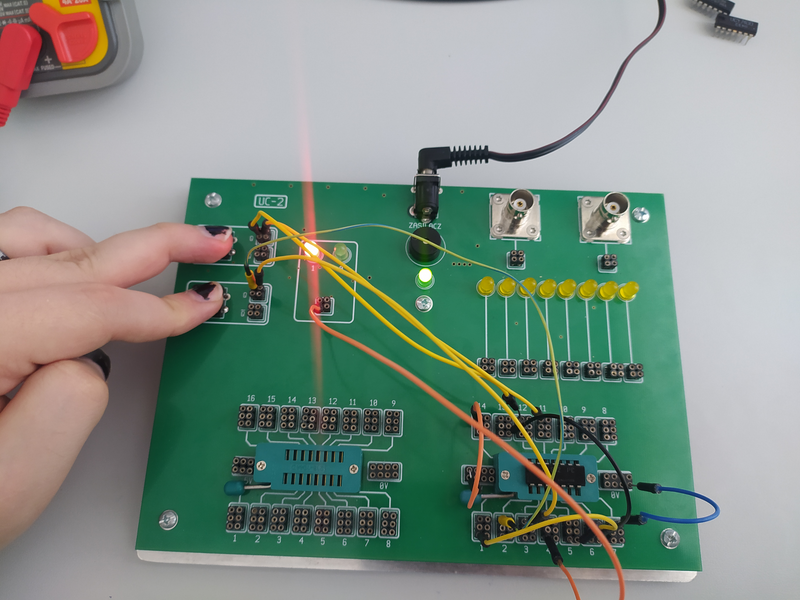
\includegraphics[width=\textwidth]{img/NOR/funkcje/1652306732382_scaled.png}
                        \end{subfigure}
                    \label{NOR:testy_AND}
                \end{figure}
            \item Tabela stanów:
                \begin{center}
                    \label{NOR:tabela_prawdy_AND}
                    \begin{tabular}{|c|c|>{\columncolor[gray]{0.8}}c|}
                        \hline
                        A & B & Y \\
                        \hline
                        0 & 0 & 0 \\
                        \hline
                        0 & 1 & 0 \\
                        \hline
                        1 & 0 & 0 \\
                        \hline
                        1 & 1 & 1 \\
                        \hline
                    \end{tabular}
                \end{center}
            \item Zbudowany układ \textbf{poprawnie} reaguje na przesyłane sygnały (zgodnie z teoretycznymi przewidywaniami \ref{tabela_prawdy:AND})
        \end{itemize}
